\subsubsection{Physical Database Design}

\begin{figure}[H]
    \centering
    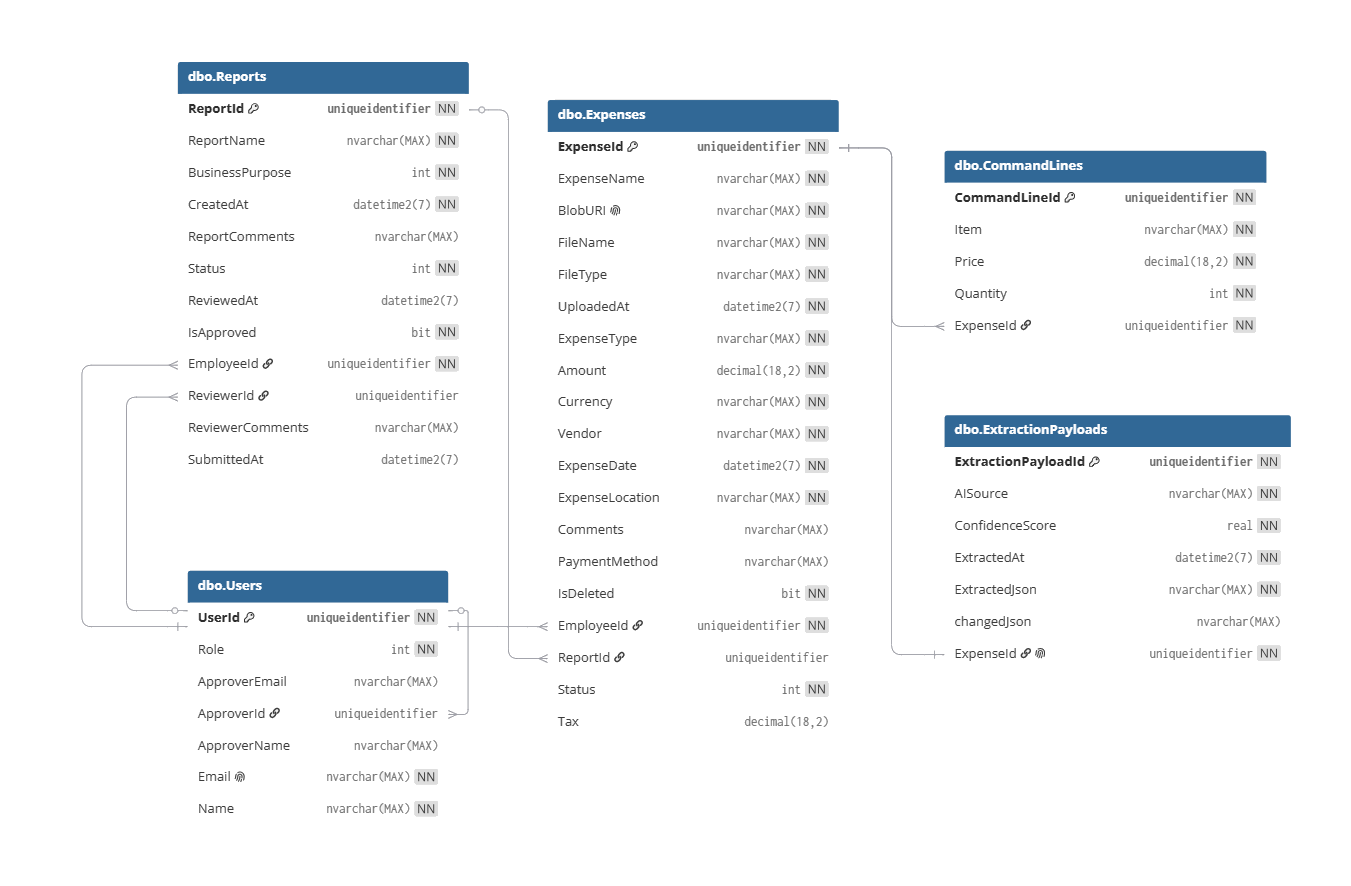
\includegraphics[width=\textwidth]{Images/DB/DBArch.png}
    \caption[Database schema diagram]
    {Database schema diagram. [Own creation]}
    \label{fig:database-schema-diagram}
\end{figure}

The physical database design is shown in the schema above (Figure \ref{fig:database-schema-diagram}). While the logical design defines the structure, the physical design focuses on performance. To ensure fast query performance, indexes are critical. Entity Framework Core automatically creates indexes on all primary keys and foreign keys. These indexes cover the most common query patterns, such as retrieving all expenses belonging to a specific report.
 